

\newpage
\chapter{The event generation procedure}
\label{sect:proc}
\mbox{}\vspace{-\baselineskip}



\section {The generation of the kinematical variables and the Fermi momentum}
\label{sect:gen_var}

For each event the values of all kinematical variables $W$, $Q^2$, $S_{12}$, $S_{23}$, $cos \theta_{h}$, $\phi_{h}$, $\alpha_{h}$ are generated randomly exactly in the same way as it is described in Sect~3.1 of the report~\cite{twopeg}.

\begin{figure}[!ht]
\begin{center}
\framebox{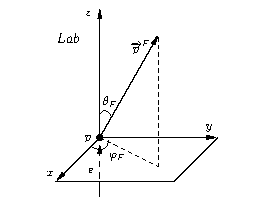
\includegraphics[width=8cm]{pictures/lab_fermi.pdf}}
\end{center}
\caption{\small The initial conditions of the reaction in the Lab frame. The incoming electron scatters off the proton that moves with the momentum $\protect\overrightarrow{p}^{F}$. }
\label{fig:lab_fermi}
\end{figure}



The simulation of the initial proton motion is performed under the following assumptions. 

\begin{itemize}
\item The Lab frame no longer corresponds to the system, where the target proton is at rest. The target proton moves in the Lab frame with the Fermi momentum as it is shown in Fig.~\ref{fig:lab_fermi}. The axis orientation in the Lab frame is the following: $Z_{lab}$ -- along the beam, $Y_{lab}$ -- up, and $X_{lab}$ -- along $[\vec Y_{lab} \times \vec Z_{lab}]$. 

\item The generated value of $W$ is treated as the smeared one calculated from the initial particle four-momenta according to Eq.~\eqref{W_fin_1} under the target-at-rest assumption (see explanation in Sect.~\ref{sec:data_an_on_mov_p}). Hereinafter this generated value is denoted as $W_{sm}$. The boundaries of the generated $Q^{2}$ versus $W_{sm}$ distribution are set according to Eqs.~\eqref{eq:kin_lim} and~\eqref{eq:kin_lim2} with $E_{beam}$ defined in the Lab frame.

\item The generated value of $Q^{2}$ is treated as the actual $Q^{2}$ value of the reaction. 
%No changes in the photon virtualities due to the motion of the initial proton are considered.



\item The four momentum of the incoming electron in the Lab frame is 

\begin{equation}
\begin{aligned}\label{mom_e_ini}
P_{e}^{Lab} = (0, 0, E_{beam}, E_{beam}),
\end{aligned}
\end{equation}
where $E_{beam}$ is the energy of the incoming electron beam that is given as an input parameter.



\item The four-momentum of the scattered electron is defined in the Lab frame exactly in the same way as it is done in the report~\cite{twopeg} (see Eqs.~\eqref{eq:el_in_lab} here as well as Eqs.~(3.2) in the report~\cite{twopeg}). 

\begin{equation}
\begin{split}\label{eq:el_in_lab}
  \nu &= \frac{W_{sm}^2+Q^2-m_{p}^{2}}{2m_{p}}\\
  E_{e'} &= E_{beam}-\nu\\
 \theta_{e'} &= acos\left (1-\frac{Q^2}{2E_{beam}E_{e'}}\right )\\
P_{e'}^{Lab} = (E_{e'}sin \theta_{e'}cos \varphi_{e'}&,E_{e'}sin \theta_{e'}sin \varphi_{e'},E_{e'}cos \theta_{e'},E_{e'}).
\end{split}
\end{equation}

Here $\nu$ is the virtual photon energy in the Lab frame, $m_{p}$ the target proton mass, and $E_{e'}$ and $\theta_{e'}$ the scattered electron energy and polar angle, respectively. $W_{sm}$, $Q^2$, and $\varphi_{e'}$ are the generated reaction invariant mass, the photon virtuality, and the azimuthal angle of the scattered electron, respectively.

%The electron defined by Eq.~\ref{eq:el_in_lab} is treated as the actual scattered electron registered after the reaction of double pion electroproduction on the moving proton has happened.

The electron defined by Eqs.~\eqref{eq:el_in_lab} imitates the actual scattered electron experimentally registered after the reaction of double-pion electroproduction off the moving proton has happened.




\end{itemize}

The components of the initial proton three-momentum $p_{x}^{F}$, $p_{y}^{F}$, and $p_{z}^{F}$ are generated randomly\footnote[1]{The algorithm of generating the initial proton three-momentum is coded in the subroutine \textit{fermi\_bonn.cxx}.} according to the Bonn potential~\cite{Machleidt:1987hj}. The four-momentum of the initial proton in the Lab frame is then determined by




\begin{equation}
\begin{aligned}\label{mom_p_ini}
P_{p}^{Lab} = (p_{x}^{F}, p_{y}^{F}, p_{z}^{F}, \sqrt{m_{p}^{2}+[p_{x}^{F}]^{2}+[p_{y}^{F}]^{2}+[p_{z}^{F}]^{2}}).
\end{aligned}
\end{equation}

The actual value of the invariant mass of the final hadron system is then determined by\footnote[2]{The determination of $W_{true}$ according to Eq.~\eqref{w_fermi_nonsm} distorts the flatness of the unweighted event distribution of $W_{true}$. This question is addressed in Sect.~\ref{sect:weights}.}



\begin{equation}
\begin{aligned}\label{w_fermi_nonsm}
W_{true}=\sqrt{(P^{Lab}_{p}+P_{\gamma_{v}}^{Lab})^{2}},
\end{aligned}
\end{equation}
where $P^{Lab}_{p}$ is the four-momentum of the moving initial proton defined by Eq.~\eqref{mom_p_ini} and $P_{\gamma_{v}}^{Lab}=P_{e}^{Lab}-P_{e'}^{Lab}$ the four-momentum of the virtual photon with $P_{e}^{Lab}$ and $P_{e'}^{Lab}$ the four-momenta of the incoming and scattered electrons defined by Eqs.~\eqref{mom_e_ini} and~\eqref{eq:el_in_lab}, respectively. 

The components of the initial proton three-momentum are generated under the condition $W_{true}>1.2375$~GeV thus demanding the actual invariant mass of the final hadronic system to be greater than the double-pion production threshold.



The scope of Fermi smearing of $W$ is illustrated in Fig.~\ref{fig:w_smear}, which shows the unweighted distribution of $W_{true}$ for the fixed value of $W_{sm} =1.5$~GeV (marked by the solid vertical line). The red curve stands for the Gaussian fit, while the dashed vertical lines mark the values $W_{sm}\pm3\sigma$ to illustrate the distribution's spread. It is seen that the majority of events deviates from the value $W_{sm} =1.5$~GeV within 75~MeV.
\begin{figure}[!ht]
\begin{center}
\framebox{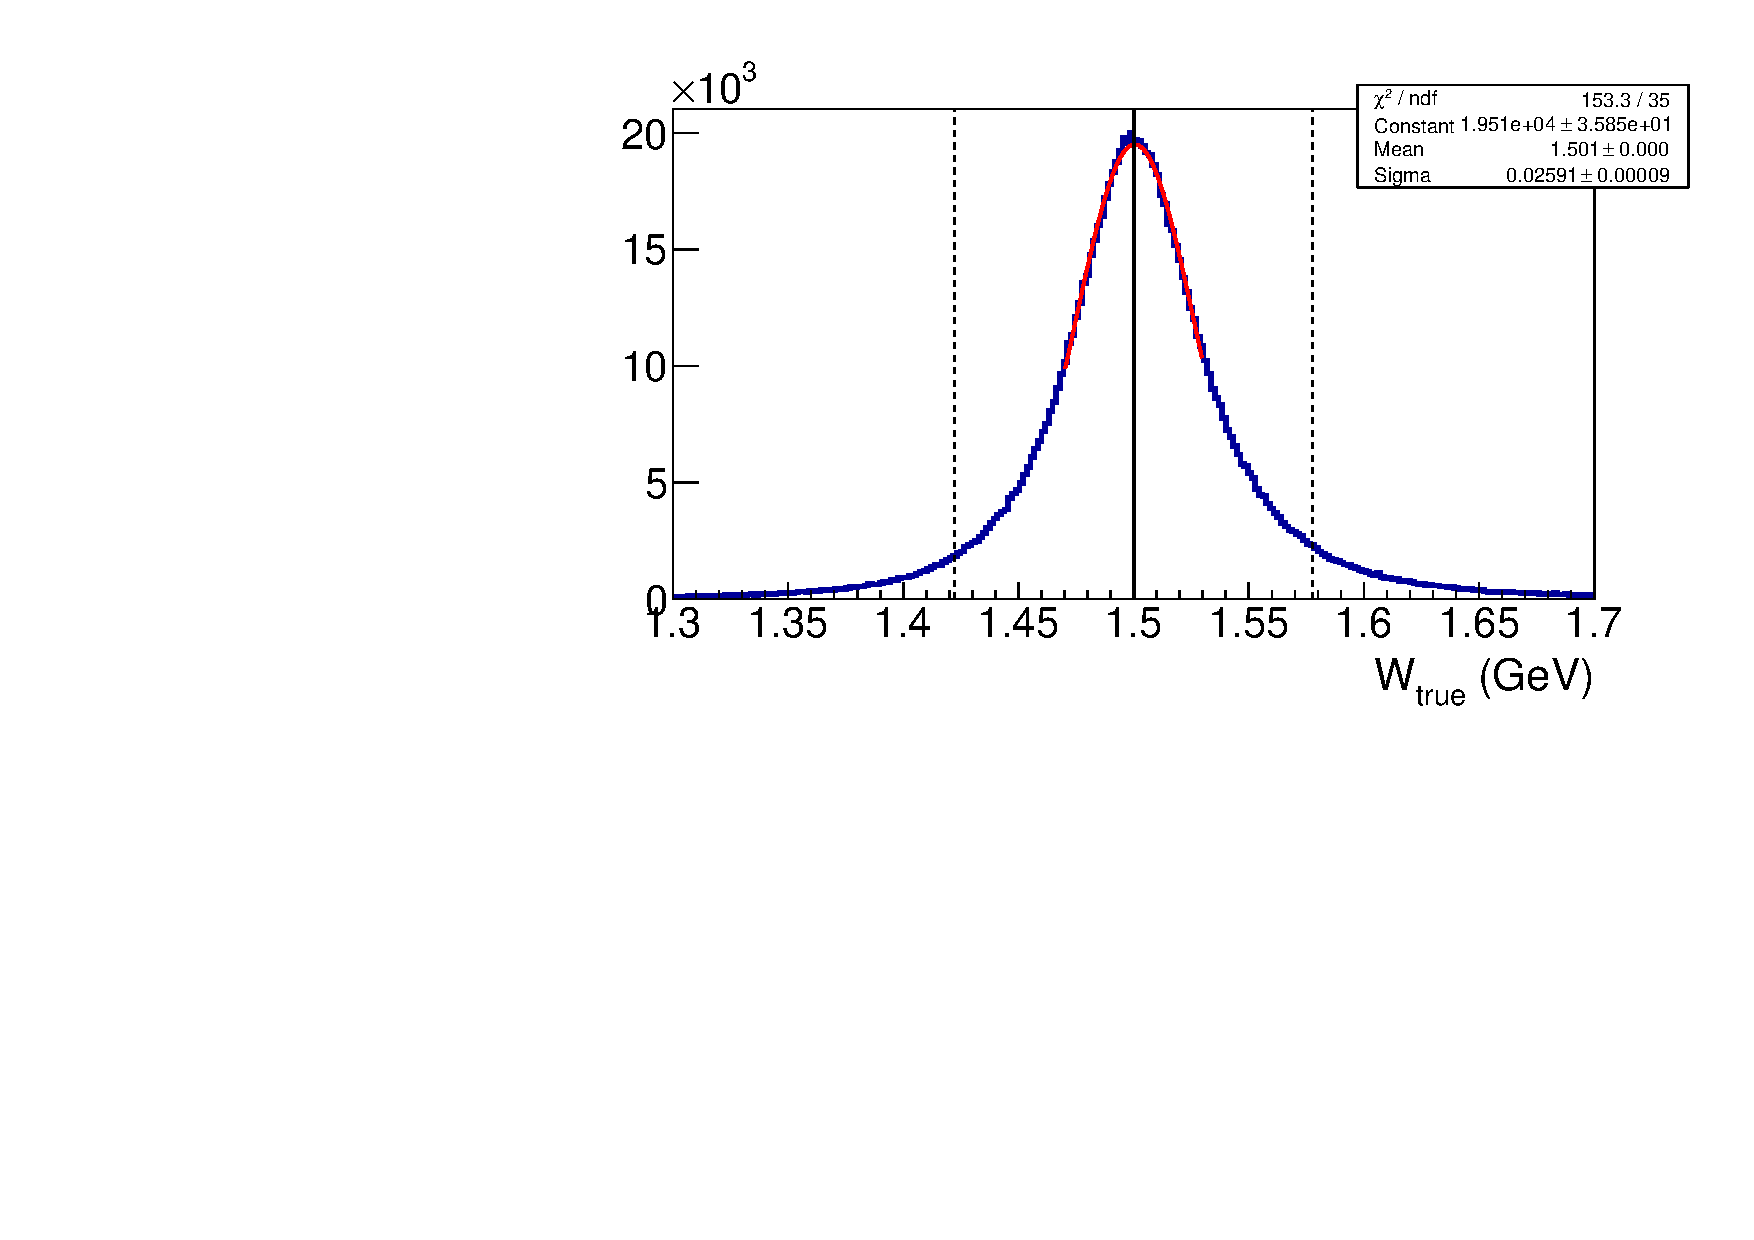
\includegraphics[width=8.8cm]{pictures/plot_w_smearing.pdf}}
\end{center}
\caption{\small The unweighted distribution of $W_{true}$ for the fixed value of $W_{sm} =1.5$~GeV (marked by the solid vertical line). The red curve stands for the Gaussian fit, while the dashed vertical lines mark the values $W_{sm}\pm3\sigma$ to illustrate the distribution's spread. The example is given for $E_{beam} = 2$~GeV and 0.4~GeV$^2$ $< Q^{2}<$ 0.5~GeV$^2$.}
\label{fig:w_smear}
\end{figure}






\section{Obtaining the particle four-momenta in the Lab frame}


The generated values of the kinematical variables should be used to obtain the four-momenta of all final particles in the Lab frame. For the case of the free proton target the recipe for this is described in Sect.~3.2 of the report~\cite{twopeg} . However, it can not be straightforwardly used for the case of the reaction off the moving proton. Therefore the following multistage method has been developed.


\begin{enumerate}[I.]
\item The four-momenta of the initial particles should be transformed from the Lab frame to the specific system, where the target proton is at rest, while the incoming electron moves along the $Z$-axis. This system hereinafter is denoted as ``quasi-Lab". The initial conditions of the reaction in the quasi-Lab frame imitate those existing in the Lab frame in the case of the free proton experiment. This circumstance determines the name choice ``quasi-Lab" that was assigned to this system\footnote[3]{The transformation of the initial particle four-momenta to the quasi-Lab frame is coded in the subroutine \textit{fermi\_rot.cxx}.}.
\item The procedure described in Sect.~3.2 of the report~\cite{twopeg} should be applied in order to obtain the four-momenta of the final particles in the quasi-Lab frame.
\item The four-momenta of the final particles should be transformed from the quasi-Lab system to the conventional Lab frame\footnote[4]{The transformation of the final particle momenta from the quasi-Lab frame to the Lab system is coded in the subroutine \textit{fermi\_anti\_rot.cxx}.}.
\end{enumerate}

Each step of this method is described below in more details.


\subsection{Obtaining the initial particle four-momenta in the quasi-Lab frame}
\label{sect:transf}

The four-momenta of the initial particles defined by Eqs.~\eqref{mom_e_ini} to~\eqref{mom_p_ini} should be transformed from the Lab frame to the quasi-Lab. This transition is performed via three steps, which are schematically shown by the green arrows in Fig.~\ref{fig:transf_proc}. These steps are described below.

%Then the four-momenta of the initial particles defined by Eq.~\eqref{mom_e_ini}, Eq.~\eqref{eq:el_in_lab} and Eq.~\eqref{mom_p_ini} should be transformed from the Lab frame to the specific system, where the target proton is at rest, while the initial electron moves along $Z$-axis. This system hereinafter is denoted as ``quasi-Lab". The transition from Lab to quasi-Lab is performed via three steps, which are schematically shown by the green arrows in Fig.~\ref{fig:transf_proc}. These steps are described below\footnote[1]{In all derivations the energy is assumed to be the last component of the four-momentum and the four-momentum to be a row vector}.

\begin{figure}[!ht]
\begin{center}
\framebox{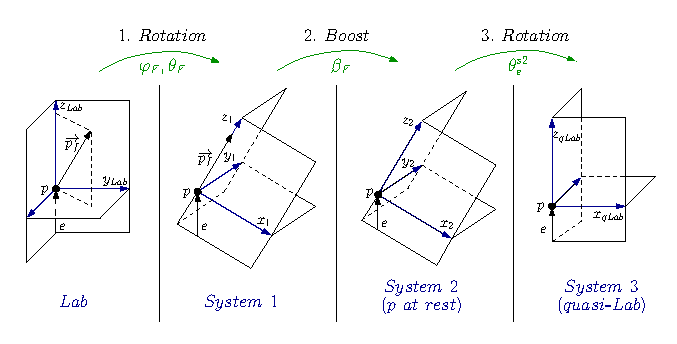
\includegraphics[width=16.5cm]{pictures/tranfs_proced.pdf}}
\end{center}
\caption{\small Schematical representation of the transformation from the Lab frame to the specific system, where the target proton is at rest, while the incoming electron moves along the $Z$-axis. This system is denoted as ``quasi-Lab". The transformation proceeds via three steps, which are shown by the green arrows.   }
\label{fig:transf_proc}
\end{figure}



\begin{enumerate}
\item The first step is the transformation from the Lab to the auxiliary system, which is denoted in Fig.~\ref{fig:transf_proc} as ``System 1" and represents the frame that has its $Z_{1}$-axis along the target proton momentum. This transformation is performed through a set of rotations of the coordinate axis as described below. 

Firstly the polar $\theta_{F}$ and azimuthal $\varphi_{F}$ angles of the moving initial proton should be calculated in the Lab frame. These angles are marked in Fig.~\ref{fig:lab_fermi} and defined~by~Eq.~\eqref{eq:ang_f}.



\begin{equation}
\begin{aligned}\label{eq:ang_f}
\theta_{F} =&~acos\left (\frac{p_{z}^{F}}{\sqrt{[p_{x}^{F}]^{2}+[p_{y}^{F}]^{2}+[p_{z}^{F}]^{2}}}\right )\\
\widetilde{\varphi}_{F} =&~acos\left (\frac{|p_{x}^{F}|}{\sqrt{[p_{x}^{F}]^{2}+[p_{y}^{F}]^{2}}}\right )\\
\varphi_{F} = &~\begin{sqcases} 
\widetilde{\varphi}_{F},&~~if~~p_{x}^{F}>0~~and~~p_{y}^{F}>0 \\ 
\pi-\widetilde{\varphi}_{F},&~~if~~p_{x}^{F}<0~~and~~p_{y}^{F}>0 \\ 
\widetilde{\varphi}_{F}+\pi,&~~if~~p_{x}^{F}<0~~and~~p_{y}^{F}<0 \\
2\pi-\widetilde{\varphi}_{F},&~~if~~p_{x}^{F}>0~~and~~p_{y}^{F}<0  
\end{sqcases} & \\
\end{aligned}
\end{equation}


Then two subsequent rotations should be made.

The $X_{lab}$-axis is rotated by the angle $\varphi_{F}$ in the $XY$-plane (around the $Z_{lab}$-axis) to force the Fermi momentum to lay in the $XZ$-plane. This rotation translates the axis $Y_{lab}$ to $Y_{1}$ and transforms the four-momentum\footnote[5]{In all derivations the energy is assumed to be the last component of the four-momentum and the four-momentum to be a row vector.} as $P' = P \cdot R_{\varphi_{F}}(\varphi_{F})$ with

\begin{equation}\label{eq:rot_ph_f}
R_{\varphi_{F}}(\varphi_{F}) = \begin{pmatrix}
 cos\varphi_{F}& -sin\varphi_{F} & 0 &0 \\ 
 sin\varphi_{F}& cos\varphi_{F} &  0& 0\\ 
0 & 0 & 1 &0 \\ 
 0&  0&  0&1 
\end{pmatrix}.
\end{equation}

Then one should rotate the $Z_{lab}$-axis by the angle $\theta_{F}$ in the $XZ$-plane in order to translate the axis $Z_{lab}$ to $Z_{1}$ and direct it along the Fermi momentum. This rotation transforms the four-momentum as $P'' = P' \cdot R_{\theta_{F}}(\theta_{F})$ with
\begin{equation}\label{eq:rot_th_f}
R_{\theta_{F}}(\theta_{F})=\begin{pmatrix}
cos\theta_{F} &0  &sin\theta_{F}  &0 \\ 
 0& 1 & 0 &0 \\ 
 -sin\theta_{F} &0  &cos\theta_{F}  & 0\\ 
0 &0  & 0 &1 
\end{pmatrix}.
\end{equation}

As it is sketched in Fig.~\ref{fig:transf_proc}, the incoming electron, being transformed into the ``System 1", turns out to be located in the $XZ$-plane.

\item After that the boost from the ``System 1" to the proton rest frame, which is denoted in Fig.~\ref{fig:transf_proc} as the ``System 2" should be performed. The boost transforms the four-momentum as $P''' = P'' \cdot R_{boost}(\beta)$ with

\begin{equation}\label{eq:boost}
R_{boost}(\beta) = \begin{pmatrix}
1 &0  &0  &0 \\ 
0 &1  &0  &0 \\ 
 0&  0& \gamma  &-\gamma \beta  \\ 
 0&  0& -\gamma \beta  & \gamma 
\end{pmatrix}, \, \, \, \beta =\frac{\sqrt{[p_{x}^{F}]^{2}+[p_{y}^{F}]^{2}+[p_{z}^{F}]^{2}}}{\sqrt{m_{p}^{2}+[p_{x}^{F}]^{2}+[p_{y}^{F}]^{2}+[p_{z}^{F}]^{2}}}, \, \, \,  \textrm{and} \,\,\,   \gamma =\frac{1}{\sqrt{1-\beta ^{2}}},
\end{equation}
where $\beta$ is the magnitude and $Z$-component of the three-vector $\overrightarrow{\beta}=(0,0,\beta)$.

In ``System 2" the incoming electron is still located in the $XZ$-plane.

%After the boost the four-momenta of the final hadrons are defined in the Lab$'$ frame, which has the CMS-like axis orientation.


\item Finally, one should rotate the axis of the proton rest frame (``System 2") to find oneself in the quasi-Lab frame (``System 3"), which has its $Z_{qLab}$-axis along the incoming electron. For that purpose the polar angle of the incoming electron in the ``System 2" should be defined by

\begin{equation}
\begin{aligned}\label{eq:ang_ei_sys2}
\theta_{e}^{s2} =&~acos\left (\frac{p_{z}^{e}}{\sqrt{[p_{x}^{e}]^{2}+[p_{y}^{e}]^{2}+[p_{z}^{e}]^{2}}}\right ),\\
\end{aligned}
\end{equation}

where $p_{x}^{e}$, $p_{y}^{e}$, and $p_{z}^{e}$ are the corresponded components of the incoming electron momentum in the ``System 2".

Then the $Z_{2}$-axis should be rotated with the angle $\theta_{e}^{s2}$ in the $XZ$-plane in order to be translated into $Z_{qLab}$, which is directed along the incoming electron momentum. This rotation transforms the four-momentum as $P'''' = P''' \cdot R_{\theta_{e}^{s2}}(\theta_{e}^{s2})$  with

\begin{equation}\label{eq:rot_th_s2}
R_{\theta_{e}^{s2}}(\theta_{e}^{s2})=\begin{pmatrix}
cos\theta_{e}^{s2} &0  &-sin\theta_{e}^{s2}  &0 \\ 
 0& 1 & 0 &0 \\ 
 sin\theta_{e}^{s2} &0  &cos\theta_{e}^{s2}  & 0\\ 
0 &0  & 0 &1 
\end{pmatrix}.
\end{equation}

\end{enumerate}

After all manipulations the four-momenta of the initial particles are written in the quasi-Lab system in the following way,


\begin{equation}
\begin{aligned}\label{eq:in_part_qlab}
P_{p}^{qLab} &= (0, 0, 0, m_{p}),\\[5pt]
P_{e}^{qLab} &= (0, 0, \widetilde{E}_{beam}^{qL}, \widetilde{E}_{beam}^{qL}) \textrm{,~and} \\[5pt]
P_{e'}^{qLab} &= (E_{e'}^{qL}sin \theta_{e'}^{qL}cos \varphi_{e'}^{qL},E_{e'}^{qL}sin \theta_{e'}^{qL}sin \varphi_{e'}^{qL},E_{e'^{qL}}cos \theta_{e'}^{qL},E_{e'}^{qL}),
\end{aligned}
\end{equation}
where $\widetilde{E}_{beam}^{qL}$ is $Z$-component of the incoming electron momentum in the quasi-Lab frame, while $E_{e'}^{qL}$, $\theta_{e'}^{qL}$, and $\varphi_{e'}^{qL}$ are the energy and spatial angles of the scattered electron in the quasi-Lab frame, respectively.

%(P_{x}^{e'qLab},P_{y}^{e'qLab},P_{z}^{e'qLab},P_{z}^{e'qLab}),
As it is seen from Eqs.~\eqref{eq:in_part_qlab}, in the quasi-Lab system the target proton is at rest, the incoming electron moves along the $Z_{qLab}$-axis, while the scattered electron has a certain known orientation. Thus, the initial conditions of the reaction in the quasi-Lab system perfectly imitate those existing in the Lab system in the case of the free proton experiment. %This circumstance determines the name ``quasi-Lab" that was assigned to this system.

\begin{figure}[!ht]
\begin{center}
\framebox{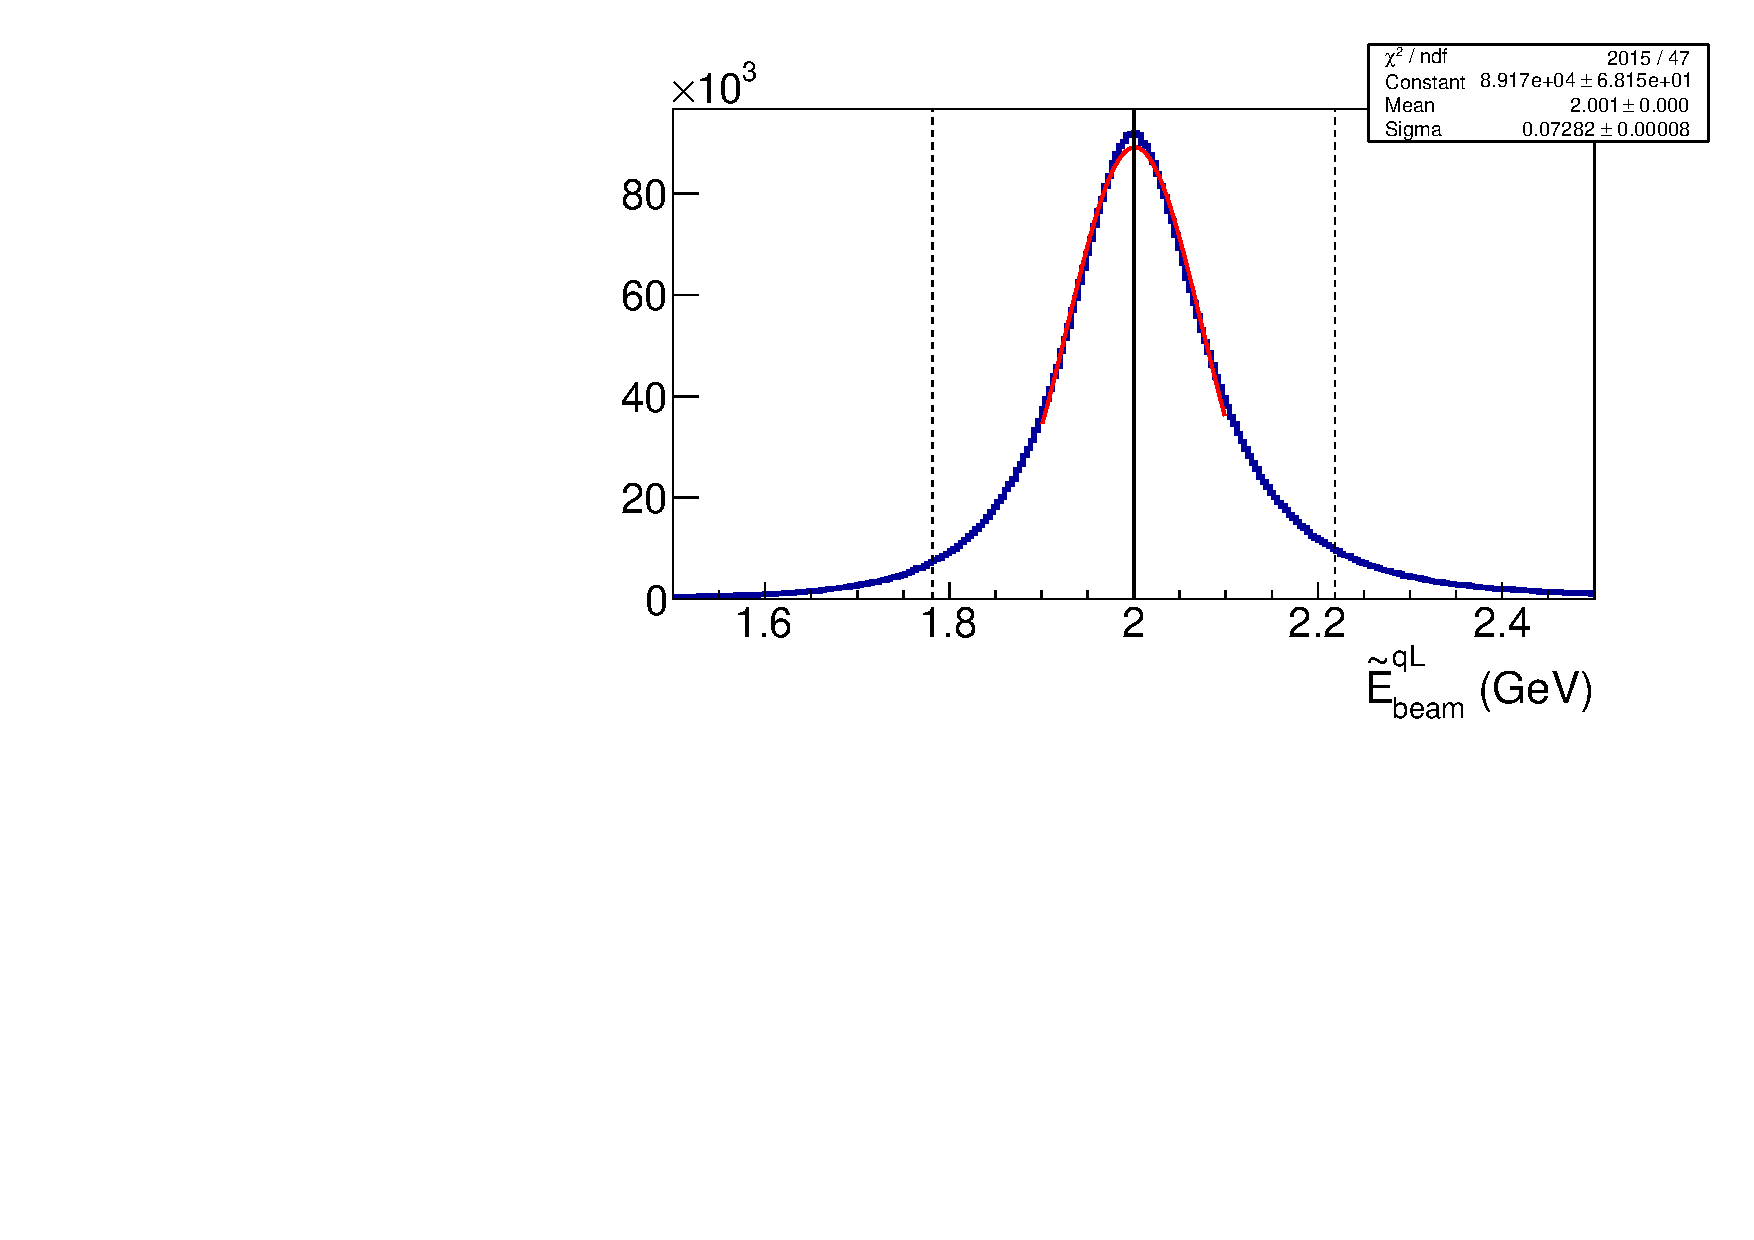
\includegraphics[width=8.8cm]{pictures/e_beam_eff.pdf}}
\end{center}
\caption{\small The distribution of the effective beam energy $\widetilde{E}_{beam}^{qL}$ defined in the quasi-Lab frame. The solid vertical line shows the value of the beam energy in the Lab frame $E_{beam} = 2$~GeV. The red curve stands for the Gaussian fit, while the dashed vertical lines mark the values $E_{beam}\pm3\sigma$ to illustrate the distribution's spread. The example is given for  1.3~GeV~$<~W_{sm}~<$~1.9~GeV and 0.4~GeV$^2$ $< Q^{2}<$ 0.5~GeV$^2$. }
\label{fig:e_beam_eff}
\end{figure}



$\widetilde{E}_{beam}^{qL}$ in Eqs.~\eqref{eq:in_part_qlab} is a so-called effective beam energy of the incoming electron in the quasi-Lab system, which does not coincide with the usual $E_{beam}$ that is defined in the Lab system and given as an input parameter. This effective beam energy is unique for each event and determined by the generated Fermi momentum.

The distribution of the effective beam energy $\widetilde{E}_{beam}^{qL}$ is shown in Fig.~\ref{fig:e_beam_eff}. The solid vertical line shows the value of the beam energy in the Lab frame $E_{beam} = 2$~GeV. The distribution is almost symmetric with respect to that line\footnote[6]{The minor asymmetry of the distribution comes from the imposed restriction $W_{true}>1.2375$~GeV.}. The red curve stands for the Gaussian fit, while the dashed vertical lines mark the values $E_{beam}\pm3\sigma$ to illustrate the distribution's spread. It is seen that for the majority of events the effective beam energy $\widetilde{E}_{beam}^{qL}$ deviates from the fixed laboratory value within 200~MeV.

As it was discussed in Sect.~\ref{sect:blur}, the alteration of the effective beam energy causes the blurring of the kinematically achievable limits of $W_{true}$ and $Q^2$. TWOPEG-D automatically takes into account this effect, since the calculation of $W_{true}$ according to Eq.~\eqref{w_fermi_nonsm} considers the effective beam energy $\widetilde{E}_{beam}^{qL}$.

Note that the actual invariant mass of the final hadron system $W_{true}$ as well as the photon virtuality $Q^{2}$, being Lorentz invariant, are not subject to any changes during the transformation described above.
%$P_{\gamma_{v}}^{Lab}=P_{e}^{Lab}-P_{e'}^{Lab}$
%\begin{equation}
%\begin{aligned}\label{eq:invar}
%W_{true}&=\sqrt{\left (P^{Lab}_{p}+P_{e}^{Lab}-P_{e'}^{Lab}\right )^{2}} = \sqrt{\left (P^{qLab}_{p}+P_{e}^{qLab}-P_{e'}^{qLab}\right )^{2}},\\[10pt]
%Q^{2} &= \left (P_{e}^{Lab}-P_{e'}^{Lab}\right )^{2} =  \left (P_{e}^{qLab}-P_{e'}^{qLab}\right )^{2}
%\end{aligned}
%\end{equation}




\subsection{Obtaining the final hadron four-momenta in the quasi-Lab frame}

The four-momenta of the final hadrons in the quasi-Lab frame are calculated by exactly the same procedure that is described in Sect.~3.2 of the report~\cite{twopeg} for the case of the free proton experiment. 
The procedure should be used as a ``black box" with the following three modifications of its input parameters.
%The following three  modifications should be however introduced.
% at the step five of the procedure.  

\begin{itemize}
\item One should use the true value of the invariant mass of the final hadron system $W_{true}$ defined by Eq.~\eqref{w_fermi_nonsm} instead of the generated value $W_{sm}$, which is assumed to be smeared.

\item Instead of the true beam energy of the experiment $E_{beam}$, which is defined in the Lab frame, the effective and for each event unique beam energy $\widetilde{E}_{beam}^{qL}$ from Eqs.~\eqref{eq:in_part_qlab} should be used. 

\item Instead of the generated azimuthal angle of the scattered electron $\varphi_{e'}$, which is assumed to be given in the Lab frame, one should use  $\varphi_{e'}^{qL}$ from Eqs.~\eqref{eq:in_part_qlab}, which is defined in the quasi-Lab frame.


\end{itemize}
 


\subsection{Obtaining the final particle four-momenta in the Lab frame}


Once the four-momenta of the final particles are obtained in the quasi-Lab frame, they should be transformed into the conventional Lab frame. For this purpose they should undergo all transformations shown in Fig.~\ref{fig:transf_proc} in the reverse order. Thus the rule of the four-momentum transformation from the quasi-Lab to Lab is 



\begin{equation}\label{eq:qlab_lab_tranf}
P^{Lab}_{i} = P^{qLab}_{i}\cdot R_{\theta_{e}^{s2}}(-\theta_{e}^{s2})\cdot R_{boost}(-\beta) \cdot R_{\theta_{F}}(-\theta_{F}) \cdot R_{\varphi_{F}}(-\varphi_{F}),
\end{equation}
where $P^{Lab}_{i}$ and $P^{qLab}_{i}$ denote the four-momenta of the particle $i$ in the Lab and quasi-Lab frames, respectively. The index $i$ corresponds to $p'$, $\pi^{+}$, $\pi^{-}$, and $e'$. Transformation matrices $R_{\theta_{e}^{s2}}$, $R_{boost}$, $R_{\theta_{F}}$, and $R_{\varphi_{F}}$ are defined by Eqs.~\eqref{eq:rot_th_s2},~\eqref{eq:boost},~\eqref{eq:rot_th_f}, and~\eqref{eq:rot_ph_f}, respectively.


%\vspace{20mm}
\begin{figure}[!ht]
\begin{center}
\framebox{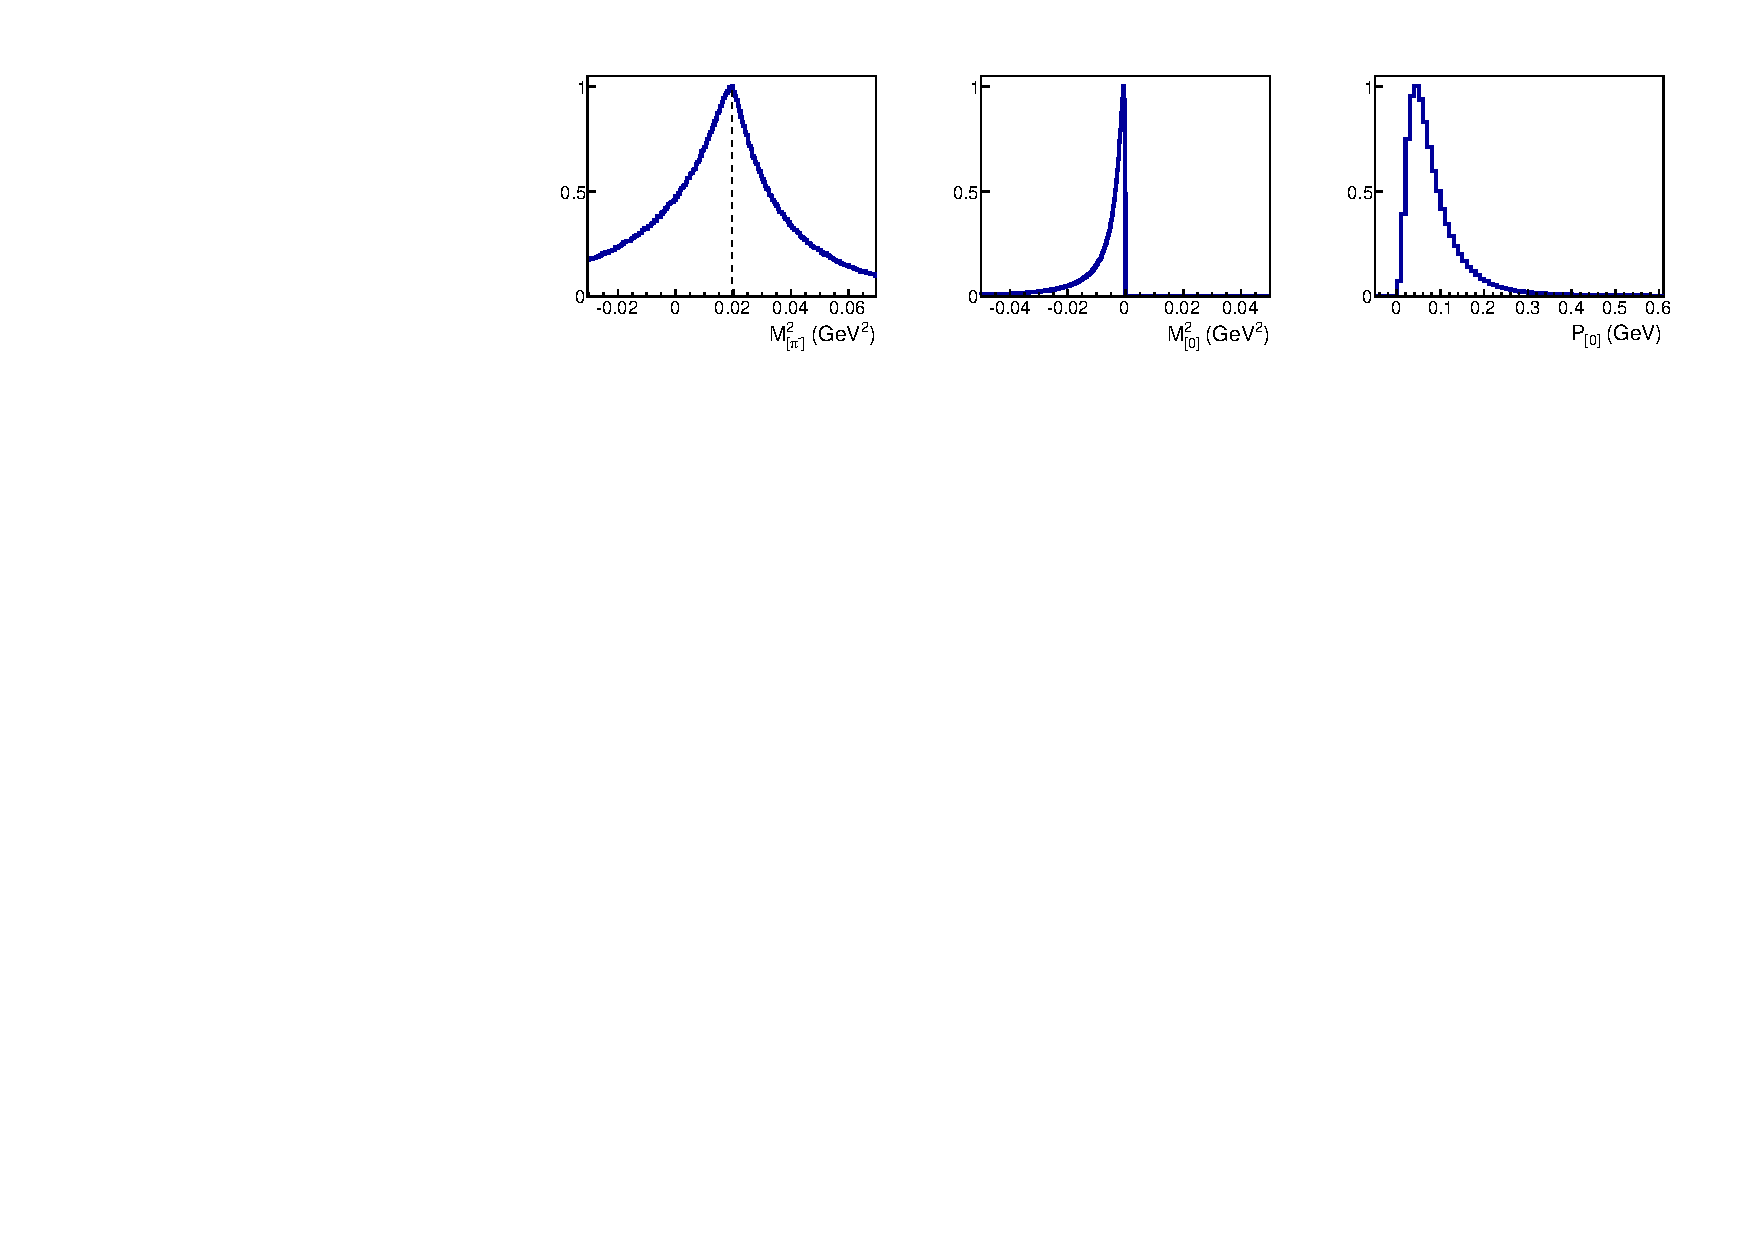
\includegraphics[width=16cm]{pictures/miss_fermi_smear.pdf}}
\end{center}
\caption{\small The distributions of the quantities $M^{2}_{[\pi^{-}]}$ (left), $M^{2}_{[0]}$ (middle), and $P_{[0]}$ (right), which are defined under the target-at-rest assumption by Eqs.~\eqref{eq:quant_targ_at_rest} and are therefore Fermi smeared. The dashed vertical line in the left plot corresponds to the pion mass squared. The example is given for $E_{beam} = 2$~GeV, 1.3~GeV $< W_{sm} <$ 1.8~GeV, and 0.5~GeV$^2$ $< Q^{2}<$ 0.7~GeV$^2$. }
\label{fig:miss_fermi_smear}
\end{figure}

Figure~\ref{fig:miss_fermi_smear} demonstrates the distributions of the quantities $M^{2}_{[\pi^{-}]}$ (left), $M^{2}_{[0]}$ (middle), and $P_{[0]}$ (right), which are defined in the following way,


\begin{equation}
\begin{aligned}\label{eq:quant_targ_at_rest}
&M^{2}_{[\pi^{-}]} &= &~~[P_{e}^{Lab}&+~&P_{p}&-~&P_{e'}^{Lab}&-~&P_{p'}^{Lab}&-~&P_{\pi^{+}}^{Lab}]^{2}&,\\[5pt]
&M^{2}_{[0]} &= &~~[P_{e}^{Lab}&+~&P_{p}&-~&P_{e'}^{Lab}&-~&P_{p'}^{Lab}&-~&P_{\pi^{+}}^{Lab}&-~&P_{\pi^{-}}^{Lab} ]^{2} \textrm{,~and}\\[5pt]
&~P_{[0]} &= &~~|\overrightarrow{P}_{e}^{Lab}&+~&\overrightarrow{P}_{p}&-~&\overrightarrow{P}_{e'}^{Lab}&-~&\overrightarrow{P}_{p'}^{Lab}&-~&\overrightarrow{P}_{\pi^{+}}^{Lab}&-~&\overrightarrow{P}_{\pi^{-}}^{Lab} |,
\end{aligned}
\end{equation}
where $P_{e}^{Lab}$ and $P_{e'}^{Lab}$ are the four-momenta of the incoming and scattered electrons given by Eqs.~\eqref{mom_e_ini} and~\eqref{eq:el_in_lab}, respectively. $P_{p'}^{Lab}$, $P_{\pi^{+}}^{Lab}$, and $P_{\pi^{-}}^{Lab}$ are the four-momenta of the final hadrons determined by the method described above, while $P_{p}=(0,0,0,m_{p})$ is the four-momentum of the target proton under the target-at-rest assumption. The vectors indicate the corresponding three-momenta.

Equation set~\eqref{eq:quant_targ_at_rest} defines $M^{2}_{[\pi^{-}]}$, $M^{2}_{[0]}$, and $P_{[0]}$ under the target-at-rest assumption in order to imitate the conditions of the real experiment, where the target proton momentum may be not known.  The distributions in Fig.~\ref{fig:miss_fermi_smear}  demonstrate therefore Fermi smearing. The quantity $P_{[0]}$ shown in the right plot, being the missing momentum of the target proton, is distributed according to the Bonn potential~\cite{Machleidt:1987hj}. 























  

